\documentclass[a4paper,onecolumn,11pt]{doofus}

\usepackage{tikz}

\title{\texttt{MPMbox}}

\doofustitle{Reference of \texttt{MPMbox}}
\doofussubtitle{Material Point Method}
\doofusauthor{Vincent Richefeu}
\doofusdate{}
\doofuslogo{./mpmxdem_logo.png} % Optional, remove or leave empty


\usepackage{comment}
\usepackage{amsmath}


\newenvironment{codeblock}
  {\par\vspace{0.75em}}
  {\par\vspace{0.75em}}

\setlength{\parindent}{0pt} % noindent

\begin{document}

\makedoofustitle

\begin{abstract}
TODO
\end{abstract}

\setcounter{tocdepth}{2}
\tableofcontents
\newpage


\section{Syntax for files \texttt{input.txt} or \texttt{conf}$\langle n \rangle$\texttt{.txt}}

\subsection{Simulation core settings}

\begin{itemize}
\item \syntax{\keyword{dt} \type{(double)}\param{value}} Time step increments.
\item \syntax{\keyword{t} \type{(double)}\param{value}} Current time 
\item \syntax{\keyword{finalTime} \type{(double)}\param{value}} Final time at which the simulation will stop
\end{itemize}

\subsection{Node grid}

In MPMbox, the fixe grid can only be regular. It can be set with the command  \syntax{\keyword{set\_node\_grid}} to allocate the nodes. Depending on the token that follows the command, the parameters used to set the grid differ. The options are:  \syntax{\keyword{Nx.Ny.lx.ly}}, \syntax{\keyword{W.H.lx.ly}} or \syntax{\keyword{W.H.Nx.Ny}}. Note that the bottom-left corner is placed at the origine $O(0,\, 0)$.\\

\begin{center}
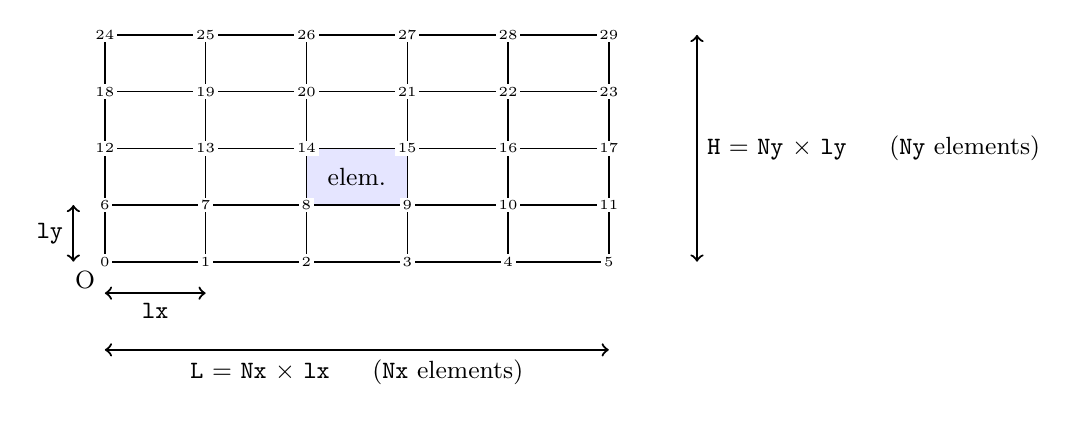
\begin{tikzpicture}[scale=0.8, every node/.style={font=\small}]

  \def\cols{5}
  \def\rows{4}
  \def\cellx{1.6}
  \def\celly{0.9}
  
  \pgfmathtruncatemacro{\lastcol}{\cols-1}
  \pgfmathtruncatemacro{\lastrow}{\rows-1}

  \draw[thick] (0,0) rectangle ({\cols*\cellx}, {\rows*\celly});

  \foreach \x in {1,...,\lastcol} {
    \draw ({\x*\cellx},0) -- ({\x*\cellx},{\rows*\celly});
  }

  \foreach \y in {1,...,\lastrow} {
    \draw (0,{\y*\celly}) -- ({\cols*\cellx},{\y*\celly});
  }

  \draw[fill=blue!10] (2*\cellx,1*\celly) rectangle (3*\cellx,2*\celly);
  \node at (2.5*\cellx,1.5*\celly) {elem.};

  \draw[<->, thick] (0,-1.4) -- (\cols*\cellx,-1.4)
    node[midway, below] {\texttt{L} = \texttt{Nx} $\times$ \texttt{lx} $\quad$ (\texttt{Nx} elements)};
  \draw[<->, thick] (\cols*\cellx+1.4,0) -- (\cols*\cellx+1.4,\rows*\celly)
    node[midway, right] {\texttt{H} = \texttt{Ny} $\times$ \texttt{ly} $\quad$ (\texttt{Ny} elements)};

  \draw[<->, thick] (0, -0.5) -- (\cellx, -0.5) node[midway, below] {\texttt{lx}};
  \draw[<->, thick] (-0.5, 0) -- (-0.5, \celly) node[midway, left] {\texttt{ly}};
  \node[below left] (0.1, 0.1)  {O};
  
  \pgfmathtruncatemacro{\nx}{\cols+1}
  \pgfmathtruncatemacro{\ny}{\rows+1}
  \pgfmathtruncatemacro{\numnodes}{\nx*\ny}

  \pgfmathtruncatemacro{\nodeid}{0}
  \foreach \j in {0,...,\rows} {%
    \foreach \i in {0,...,\cols} {%
      \pgfmathtruncatemacro{\nodeid}{\j*(\cols+1) + \i}
      \node[fill=white, inner sep=1pt] at ({\i*\cellx}, {\j*\celly}) {\tiny \nodeid};
    }%
  }
\end{tikzpicture}
\end{center}

% example

Some data in the nodes are stored with the conf-file (after the nodes have been set, for example with the command \syntax{\keyword{set\_node\_grid}}). The syntax is as follows:
\begin{codeblock}
\syntax{\keyword{Nodes} \type{(int)}\param{nbNodes}} \\
$\Big[$ \syntax{\type{(int)}\param{nodeId} \type{(vec2r)}\param{q} \type{(vec2r)}\param{f} \type{(vec2r)}\param{fb} \type{(double)}\param{mass} \type{(0/1)}\param{xfixed} \type{(0/1)}\param{yfixed}} $\Big]_{\times \text{\param{nbNodes}}}$ 
\end{codeblock}

% [...]

The $x$ and/or $y$ velocity components can be assigned to nodes on a line-by-line or column-by-column basis:
%
\begin{codeblock}
\syntax{\keyword{set\_BC\_column} \type{(int)}\param{column\_num} \type{(int)}\param{line0} \type{(int)}\param{line1} \type{(0/1)}\param{Xfixed}  \type{(0/1)}\param{Yfixed} } \\
\syntax{\keyword{set\_BC\_line} \type{(int)}\param{line\_num} \type{(int)}\param{column0} \type{(int)}\param{column1} \type{(0/1)}\param{Xfixed}  \type{(0/1)}\param{Yfixed} } 
\end{codeblock}

\begin{center}
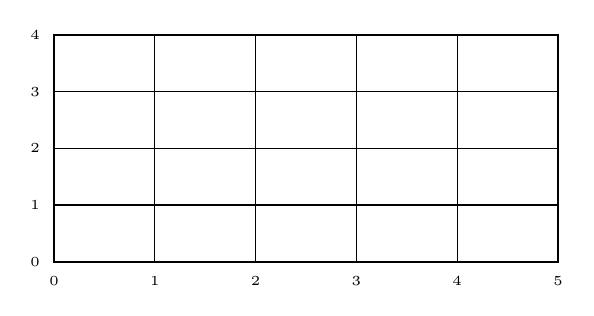
\begin{tikzpicture}[scale=0.8, every node/.style={font=\small}]

  \def\cols{5}
  \def\rows{4}
  \def\cellx{1.6}
  \def\celly{0.9}
  
  \pgfmathtruncatemacro{\lastcol}{\cols-1}
  \pgfmathtruncatemacro{\lastrow}{\rows-1}

  \draw[thick] (0,0) rectangle ({\cols*\cellx}, {\rows*\celly});

  \foreach \x in {1,...,\lastcol} {
    \draw ({\x*\cellx},0) -- ({\x*\cellx},{\rows*\celly});
  }
  
   \foreach \x in {0,...,\cols} {
    \node[fill=white, inner sep=1pt] at ({\x*\cellx},-0.3) {\tiny \x};
  }

  \foreach \y in {1,...,\lastrow} {
    \draw (0,{\y*\celly}) -- ({\cols*\cellx},{\y*\celly});
  }
  
  \foreach \y in {0,...,\rows} {
    \node[fill=white, inner sep=1pt] at (-0.3,{\y*\celly}) {\tiny \y};
  }

\end{tikzpicture}
\end{center}


\subsection{Shape functions}


\syntax{\keyword{ShapeFunction} \type{(string)}\param{shapeFunction}}


%**`ShapeFunction`** (_string_)shapeFunction
%shapeFunction can be either `Linear`, `RegularQuadLinear` or `BSpline`


\subsection{Constitutive Models}


Before using a constitutive model, you must first create one by assigning it an identifier, specifying the model type, and providing the corresponding parameters.

\begin{codeblock}
\syntax{\keyword{model} \type{(string)}\param{modelIdentifier} \type{(string)}\param{modelName} (...list of parameters...)}
\end{codeblock}

Each material point will then be associated with the model through its identifier.
Here are the lists of parameters for each \syntax{\param{modelName}}:
\begin{itemize}
\item  \syntax{\keyword{HookeElasticity}}: \syntax{\type{(double)}\param{Young} \type{(double)}\param{Poisson}}
\item  \syntax{\keyword{VonMisesElastoPlasticity}}: \syntax{\type{(double)}\param{Young} \type{(double)}\param{Poisson} \type{(double)}\param{PlasticYieldStress}}
\item  \syntax{\keyword{MohrCoulomb}}: \syntax{\type{(double)}\param{Young} \type{(double)}\param{Poisson} \type{(double)}\param{FrictionAngle}}\\ 
\syntax{\type{(double)}\param{Cohesion} \type{(double)}\param{DilatancyAngle}}
\item  \syntax{\keyword{CHCL\_DEM}}: \syntax{\type{(string)}\param{conf-filename}}
\end{itemize}


\subsection{Adding material points}


Material points can be added by placing them on a grid. The corresponding command in this case is: \\

\begin{codeblock}
 \syntax{\keyword{set\_MP\_grid} \type{(int)}\param{group} \type{(string)}\param{modelIdentifier}}
\end{codeblock}

\begin{comment}
**`set_MP_polygon`** (_int_)`group`  (_int_)`nbVertices`  (_string_)`modelName`  (_double_)`massDensity` (_double_)`sizeOfBoxes`  (... (_double_)`x` (_double_)`y` ...)


**`add_MP_ShallowPath`** (_int_)group  (_int_)nbPathPoints (_double_)height (_string_)modelName (_double_)rho (_double_)size (...list of nbPathPoints (_vec2r_)point...)
\end{comment}



\begin{comment}
**`move_MP`**   (_double_)x0  (_double_)y0  (_double_)dx  (_double_)dy  (_double_)theta
> Note that a negative value of theta rotates clockwise.

**`reset_model`**  (_int_)group  (_string__)modelName  (_double_)rho  (_double_)x0 (_double_)y0 (_double_)x1 (_double_)y1
\end{comment}



%\subsection{Splitting}
%**`splitting`**  (_bool_)Active (_bool_)splitTouchingMP (_double_)SplitValue




\subsection{Obstacles (Rigid Bodies)}

%**`Obstacle`** (_string_)type (...list of parameters that depend on type...)
%List of parameters for each type:
%  - `Line`: (_double_)x0 (_double_)y0 (_double_)x1 (_double_)y1
% - `Circle`: (_vec2r_)center (_double_)R

\subsection{Boundary Force Laws}

% need to be set after the Obstacles have been set

\subsection{Spies (Processing)}

\begin{comment}
**`Spy`** (_string_)`spyName` (...list of parameters that depend on spyName...)

List of parameters for each spyName:

  - `Work`:  (_int_)`recordPeriod`  (_string_)`fileName` (_double_)`Xmin` (_double_)`Xmax` (_int_)`nbBins`
\end{comment}

\subsection{Schedulers}


\begin{comment}
**`GravityRampe`** (_vec2r_)`gravityFrom`  (_double_)`rampStart` (_vec2r_)`gravityTo` (_double_)`rampStop`

**`PICDissipation`** (*double*)`rateOfFLIP` (*double*)`endTime`

**`ReactivateCHCLBonds`**

**`RemoveMaterialPoint`**

**`RemoveObstacle`**


\end{comment}







%\begin{thebibliography}{9}
%\bibitem{ref1} Author, A. and Author, B., "Title of the paper," Journal Name, vol. 1, no. 1, pp. 1-10, Year.
%\end{thebibliography}

\end{document}
